\chapter{Architecture}

\minitoc

\subsubsection{Purpose}

The system is to be described in this chapter. This includes the main parts of the system, the architectural drivers, how they are connected together, and their collaboration. The architecture will be described through the 4+1 view model. The party members, or the stakeholders of the system, will have different concerns, so the 4+1 view model will help us describe the system for each of them, and make sure that all expectations are accounted for.  

\clearpage


\section{Architectural drivers}
The architectural drivers defines the project and its scope. 

\begin{itemize}
    \item Improving the efficiency in the chosen domain - The traditional web application system is to be improved efficiency-wise, so power users will be able to use less time on more tasks. (non-functional requirement)
    \item Proving the concept in general - Our solution should be applicable to more general problems than those described by the chosen domain. (business constraint)
    \item Minimum console functionality - The system's console should have capabilities on par with a traditional web application: Creating objects, editing objects, deleting objects, working with lists of objects.  (functional requirement)
    \item Added flexibility - The console should allow the user to perform tasks that are not possible with a web application of comparable complexity and development cost. (non-functional requirement)
    \item Console in a web context - The console should operate in a web browser environment. (technical constraint)
    \item Tolerate changes in requirements - We must use an approach that tolerates iterative changes to the demands from the customer. If new functionality is proposed and deemed likely to make the prototype more useful, it should be implemented asap. (business constraint)
    \item Delivery on time - The project must be finished on a fixed schedule. (business constraint) 
    \item Academically sound process - The project should be executed using methods that satisfy the academical context. (business constraint)
\end{itemize}


\section{Stakeholders}
The stakeholders and their concerns when it comes to the system.

\begin{itemize}
    \item Developer
    \begin{itemize}
        \item Solve the problem and deliver a system the customer will be satisfied with.
        \item Learn new technologies
        \item Get experience with project management
        \end{itemize}
    \item Customer
    \begin{itemize}
        \item Gets a working system, which satisfies the customers wants
        \item Get a usable report on the concept, which satisfies the customers wants
    \end{itemize}
    \item End user
    \begin{itemize}
        \item Improve efficiency
        \item Easy to use after some training
    \end{itemize}
\end{itemize}



\section{4+1 view model}
The 4+1 view model\cite{Kruchten}. Here the views will be described, and how they will look in our architecture. Diagrams are based on Martin Fowler's UML\cite{Fowl04}

\subsubsection{Logical View}
Describes the functionality in the system from the end users perspective. The end users will mainly be power users, wanting to perform object editing tasks efficiently. This view will be described through class, communication and sequence diagram.

\begin{figure}[h]
\centering
\includegraphics[width=6in]{image/architecture/s3/s3clientClassDiagram.png}
\caption{Client Class Diagram}
\label{figure:s3clientClassDiagram}
\end{figure}

Figure~\ref{figure:s3clientClassDiagram} The client class diagram gives an overview of the class structure of system, and how they collaborate. WILL BE CHANGED TILL LAST DELIVERY
%This sprint we made some changes to the client side to better handle and work with the new database system we introduced in this sprint. We still has a UI/Console view, for the user to work with, but the console and UI now can work more freely onto the database through commands, as seen in the "Wonsole"-class. Since the edited client and new database together made a more dynamic system, the objects the user can work with does not need to be restricted to Book and library objects. The persistence class is instead holding more dynamic versions of these. Changes done in the console is still reflected onto the UI through the Wonsole and persistence classes. The changes are pushed onto the server through a "commit"-command, instead of an automatic push done by the previously used PubNub.

\begin{figure}[h]
\centering
\includegraphics[width=3in]{image/architecture/s3/s3serverClassDiagram.png}
\caption{Client Class Diagram}
\label{figure:s3serverClassDiagram}
\end{figure}

Figure~\ref{figure:s3serverClassDiagram} The server class diagram shows how the REST api is set up. WILL BE CHANGED TILL LAST DELIVERY
%Since the PubNub no longer is a used function, it is removed from the server side also. The new database system is both a REST api and a database system, this renders the separation of REST and DBCommunicator obsolete, and lets us merge it all together into one component. 


\subsubsection{Process View}
Describes the dynamic aspect of the system, and explains how the different parts of the system will communicate at runtime. This is described with a activity diagram.

The user will ask for an object from the backend, this will be delivered to the client through the communication channel as a json object, the client will interpret this and the user can then edit it through the console, and send it back to the backend.


\subsubsection{Physical View}
Describes the system from the system engineer's perspective. And explains the physical connections between the software components. Described through a deployment diagram. 

\begin{figure}[h]
\centering
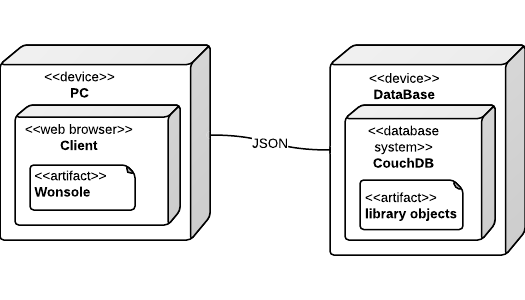
\includegraphics[width=4in]{image/architecture/s3/s3DeploymentDiagram.png}
\caption{Deployment Diagram}
\label{figure:s3DeploymentDiagram}
\end{figure}

Figure~\ref{figure:s3DeploymentDiagram} The structure of the now two different parts of the system, WILL BE CHANGED TILL LAST DELIVERY
%database can be accessed without a middleman, and the PubNub is no longer used.

\subsubsection{Development View}
Describes the system from the programmer's perspective. This will be described through how the different component parts are separated. Component and package diagrams will show this.

\begin{figure}[h]
\centering
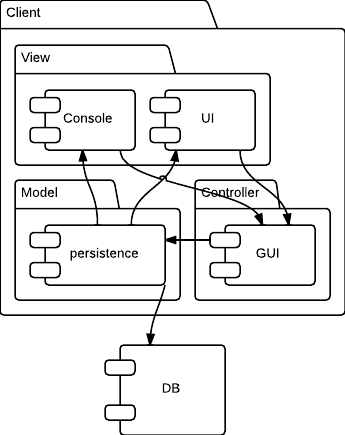
\includegraphics[width=3in]{image/architecture/s3/s3ComponentDiagram.png}
\caption{Component Diagram}
\label{figure:s3ComponentDiagram}
\end{figure}

Figure~\ref{figure:s3ComponentDiagram} These components still form a three layered structure, WILL BE CHANGED TILL LAST DELIVERY
%but the DB component is both the logical tier and the data tier. The components communicates with each other through the neighboring layer.


%\subsubsection{Scenarios}
%Describes the system through a set of use cases/scenarios. These use cases/scenarios describes how the objects and processes work together.


\section{Tactics}
The architectural tactics are used to describe how different qualities of the system are achieved. 

\subsection{Modifiability}
Anticipate changes:

Probable changes should be anticipated, and accounted for, so extending the system with new functionality should be possible. This is important since we are dealing with a prototype/proof of concept system. So the customer might change the direction we are going in through out the project, this will lead to changes, and the architecture should be able to bend after these new inputs. 

This can be handled with a well defined functionality map, so that the expected system functionalities are accounted for when the system is constructed. 


\section{Architectural patterns}
The patterns can help solve different kinds of problems with know solutions on new problems.

\subsection{Multi-tier}

The architecture of the system will be of the multi-tier kind. This means that the presentation, application processing and data management functions will be separated logically. The application (console) will translate the task of the end user, and 

The console - Translate the task of the end user.
The logical tier - Will receive the translated task from the console, and fetch information from the data storage specified by the console, and set it back to the user.
The data storage - The last tier, and it will contain the information from the library.

figure of the 3 tiers. 

\subsection{MVC}

The client gui and console communication. Since the action made in the console should be reflected in the gui and vice versa, is it natural to use a model-view-controller pattern. The information in the model will then be separated from the view (the display) and the controller which performs an update on the model. 


\subsection{Rationale}


\section{Database}
\section{GUI}

